\documentclass[border=14pt]{standalone}
\usepackage[T1]{fontenc}
\usepackage[scaled]{helvet}
\renewcommand\familydefault\sfdefault
\usepackage{tikz}
\usetikzlibrary{arrows.meta,calc,positioning}
\definecolor{personF}{HTML}{F8E0A8}\definecolor{personD}{HTML}{B8860B}
\definecolor{slackF}{HTML}{DCE8F6}\definecolor{slackD}{HTML}{5B7FA8}
\definecolor{sessF}{HTML}{CDE8E1}\definecolor{sessD}{HTML}{2E8B74}
\definecolor{subF}{HTML}{E6DDF3}\definecolor{subD}{HTML}{7E5DB8}
\definecolor{workF}{HTML}{E1EECD}\definecolor{workD}{HTML}{6A9A3A}
\definecolor{servF}{HTML}{E6E8EB}\definecolor{servD}{HTML}{8A9099}
\definecolor{codeF}{HTML}{F6DAD6}\definecolor{codeD}{HTML}{C0605A}
\definecolor{arrC}{HTML}{6B7280}\definecolor{labC}{HTML}{555B66}
\tikzset{
  box/.style={rounded corners=3pt, draw, line width=0.8pt, align=center, text width=3.4cm,
              inner sep=5pt, minimum height=1.2cm, font=\normalsize},
  person/.style={box, fill=personF, draw=personD},
  slack/.style={box, fill=slackF, draw=slackD},
  sess/.style={box, fill=sessF, draw=sessD},
  sub/.style={box, fill=subF, draw=subD},
  work/.style={box, fill=workF, draw=workD},
  serv/.style={box, fill=servF, draw=servD},
  code/.style={box, fill=codeF, draw=codeD},
  arr/.style={-{Stealth[length=2.4mm,width=1.8mm]}, draw=arrC, line width=0.8pt},
  lab/.style={font=\small\itshape, text=labC, fill=white, inner sep=1.5pt},
}
\hyphenpenalty=10000 \exhyphenpenalty=10000
\newcommand\nd[2]{\textbf{#1}\\[1pt]{\small #2}}
\newcommand\titled[2]{\node[anchor=south west, inner sep=0pt] at ($(current bounding box.north west)+(0cm,0.45cm)$)
  {{\bfseries\LARGE #1}\hspace{1.2em}{\color{labC}\large #2}};}
\begin{document}
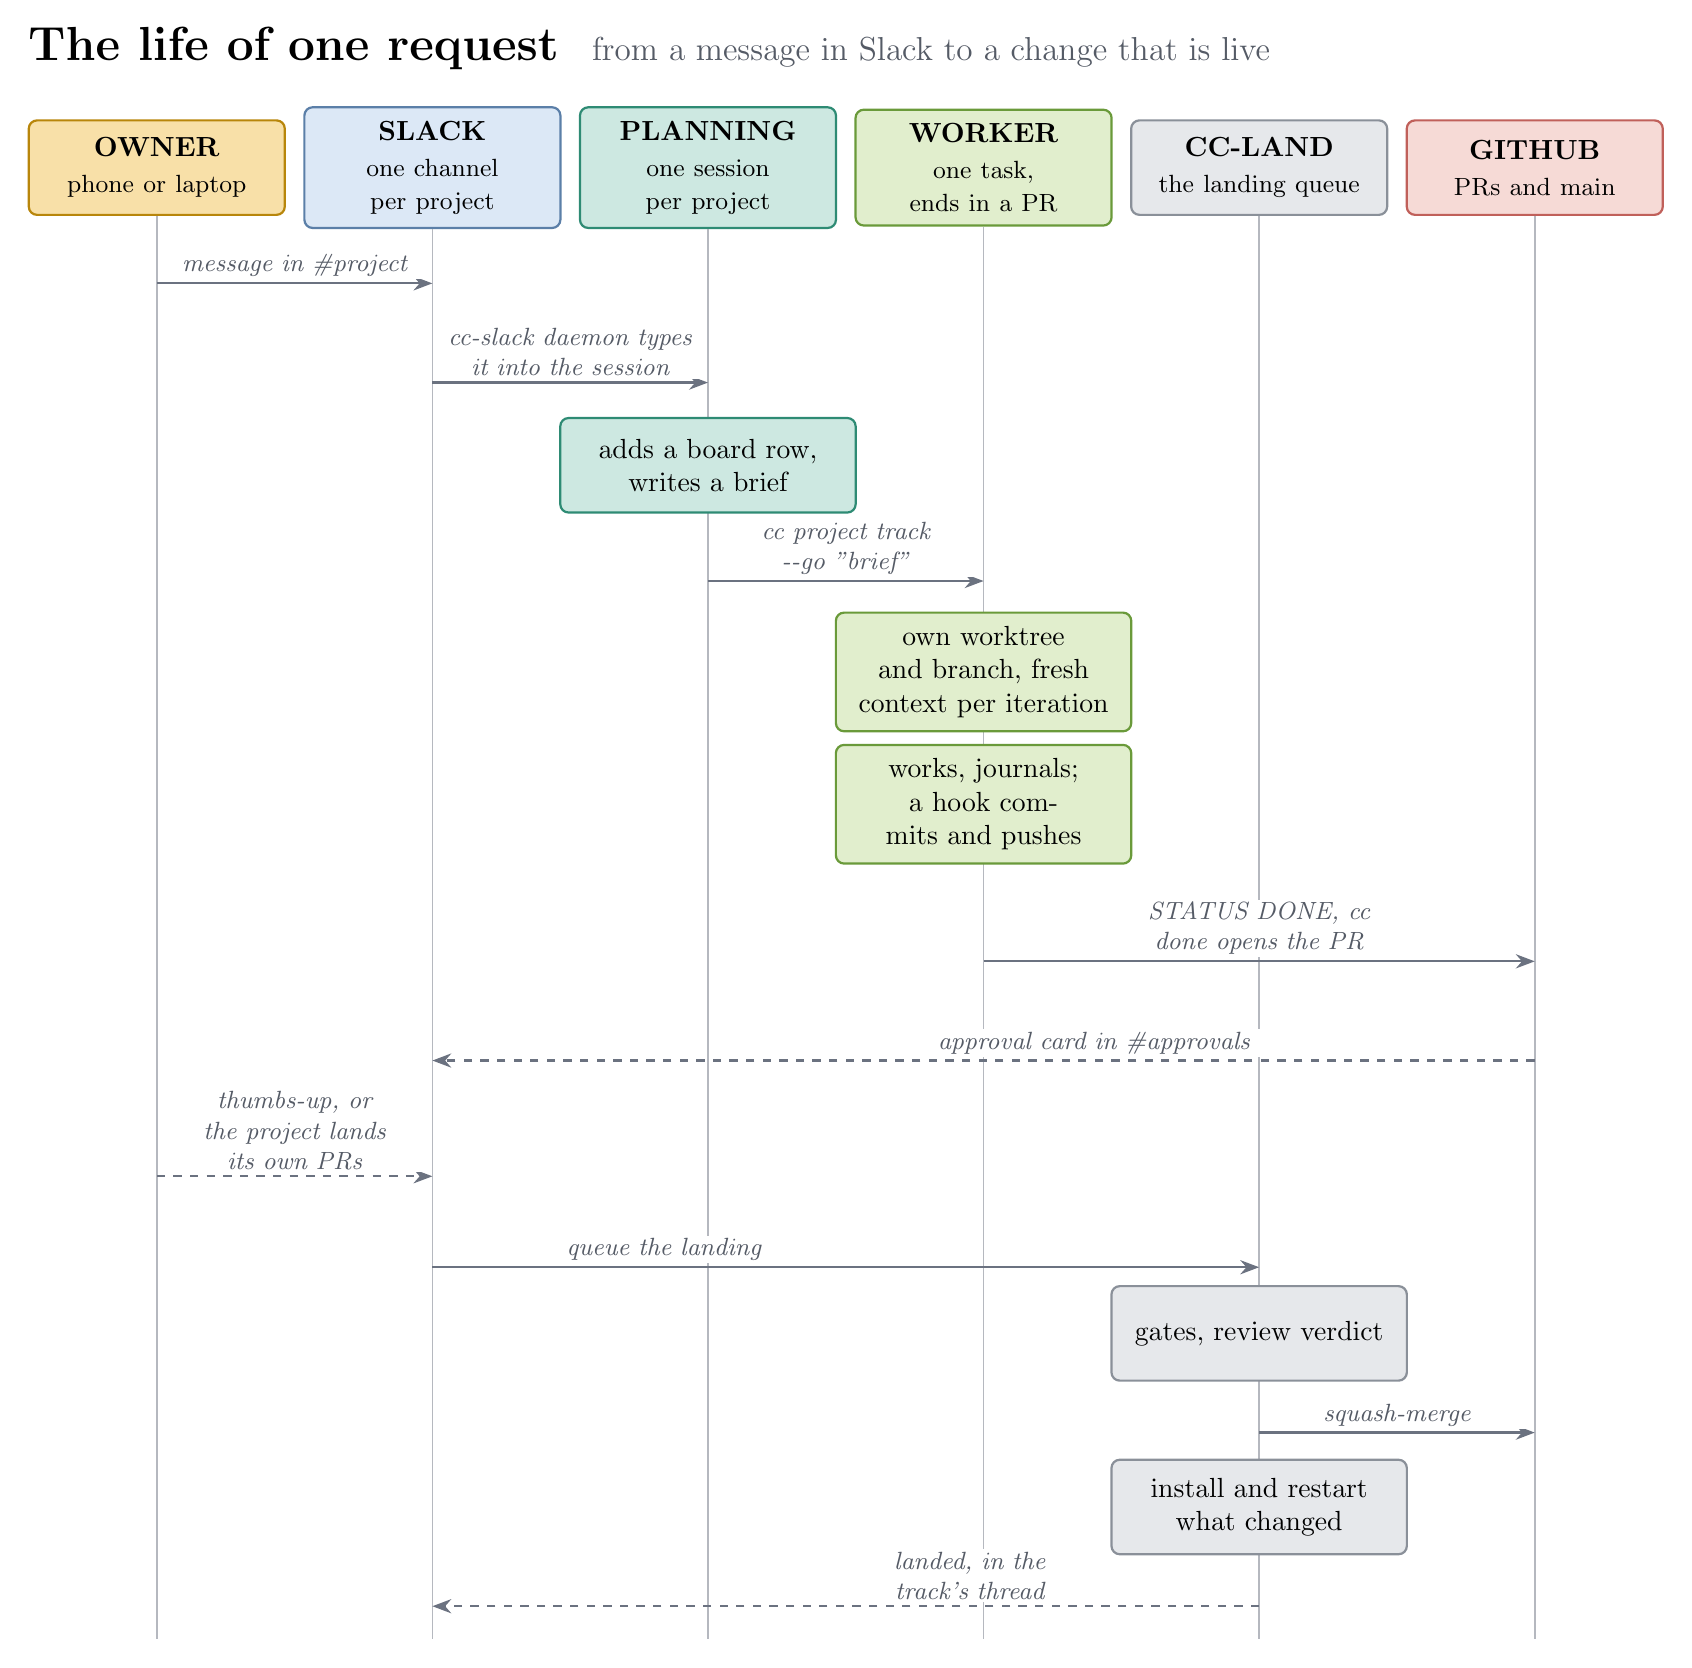
\begin{tikzpicture}[x=3.5cm, y=-1.05cm]
\tikzset{hd/.style={text width=2.9cm}, act/.style={box, text width=3.0cm, minimum height=0.8cm, font=\small, inner sep=3pt},
  msg/.style={font=\small\itshape, text=labC, align=center, text width=3.2cm, inner sep=1pt, above=1pt, fill=white},
  ret/.style={arr, dashed}}
\node[person,hd] (O) at (0,0) {\nd{OWNER}{phone or laptop}};
\node[slack,hd]  (S) at (1,0) {\nd{SLACK}{one channel per project}};
\node[sess,hd]   (P) at (2,0) {\nd{PLANNING}{one session per project}};
\node[work,hd]   (W) at (3,0) {\nd{WORKER}{one task, ends in a PR}};
\node[serv,hd]   (L) at (4,0) {\nd{CC-LAND}{the landing queue}};
\node[code,hd]   (G) at (5,0) {\nd{GITHUB}{PRs and main}};
\foreach \c in {O,S,P,W,L,G} \draw[arrC!50, line width=0.6pt] (\c.south) -- (\c.south |- 0,17.8);
% steps
\draw[arr] (0,1.4) -- node[msg] {message in \#project} (1,1.4);
\draw[arr] (1,2.6) -- node[msg] {cc-slack daemon types it into the session} (2,2.6);
\node[act, sess] at (2,3.6) {adds a board row, writes a brief};
\draw[arr] (2,5.0) -- node[msg] {cc project track -{}-go "brief"} (3,5.0);
\node[act, work] at (3,6.1) {own worktree and branch, fresh context per iteration};
\node[act, work] at (3,7.7) {works, journals; a hook commits and pushes};
\draw[arr] (3,9.6) -- node[msg, text width=4cm] {STATUS DONE, cc done opens the PR} (5,9.6);
\draw[ret] (5,10.8) -- node[msg, text width=5cm, pos=0.4] {approval card in \#approvals} (1,10.8);
\draw[ret] (0,12.2) -- node[msg, text width=3.3cm] {thumbs-up, or the project lands its own PRs} (1,12.2);
\draw[arr] (1,13.3) -- node[msg, pos=0.28] {queue the landing} (4,13.3);
\node[act, serv] at (4,14.1) {gates, review verdict};
\draw[arr] (4,15.3) -- node[msg] {squash-merge} (5,15.3);
\node[act, serv] at (4,16.2) {install and restart what changed};
\draw[ret] (4,17.4) -- node[msg, pos=0.35] {landed, in the track's thread} (1,17.4);
\titled{The life of one request}{from a message in Slack to a change that is live}
\end{tikzpicture}
\end{document}
